\documentclass[11pt]{article}

\usepackage{graphicx}

\setlength{\parindent}{0pt}

\begin{document}
\title{ELEC 221, Visual and Statistics Project}
\author{Morten Kals, 52429140}
\maketitle

\section*{Task 1}

\subsection*{Q0}
The total number of frames in the video is 3081.
The frame-rate of the video is 29.97fps. 

\subsection*{Q1}
\begin{itemize}
	\item The data-array representing each frame consists of a three-dimensional array with 720 rows, 1280 columns and three colour-channels (representing R, B and G). The array for one frame thus consist of $720\times1280\times3=2 764 800$ elements. 
	\item The height of each frame is 720 pixels and the width of each frame is 1280 pixels. 
	\item A true colour RGB image has 3 channels containing values from 0 to 255. As $2^8=256$ this means $3*8=24$ bits make up one pixel. 
\end{itemize}


\section*{Task 2}

\subsection*{Q2}
As a grayscale image only contains one colour channel, each pixel requires of 8 bits. 

\subsection*{Q3}
I used the MATLAB function rgb2gray to convert from RGB to grayscale. It works by forming a weighted sum of R, G and B components of the image. \[x=0.2989\times R+0.5870\times G+0.1140\times B\]

\subsection*{Fig. 1}
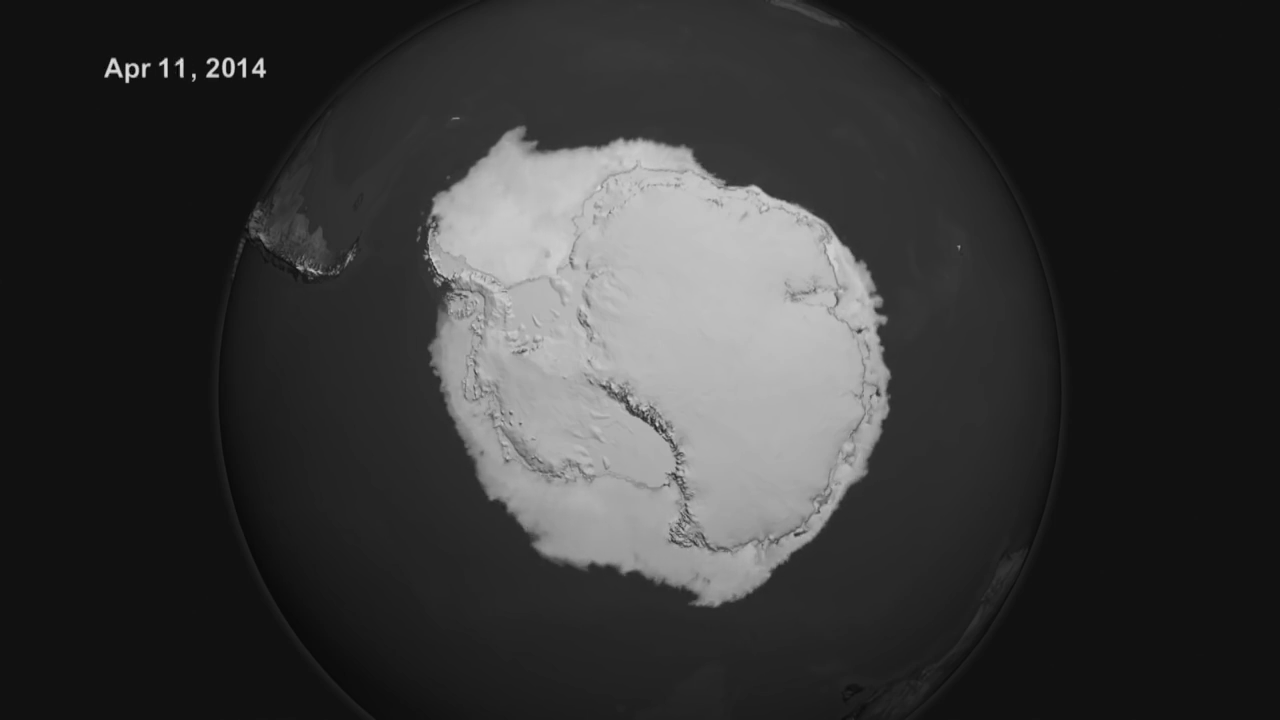
\includegraphics[width=\textwidth]{reportImages/figure1}

\subsection*{Q4}

\section*{Task 3}
\subsection*{Q5}
A grayscale image can be binarized by testing each pixel grayscale value against a threshold. If larger, the pixel is made white whereas if the value is lower the pixel is made black. The threshold can either be predefined, or dynamically calculated based on image parameters. \\

 I used the function \textit{imbinarize} which works by using a locally adaptive threshold. The functions looks at nearby pixels and compares a local mean intensity against the grayscale value of the given pixel. This ensures both light and dark regions in an images can produce black pixels using the same filter, whereas a static threshold value would have to be tuned to the individual image.

\subsection*{Fig. 2}
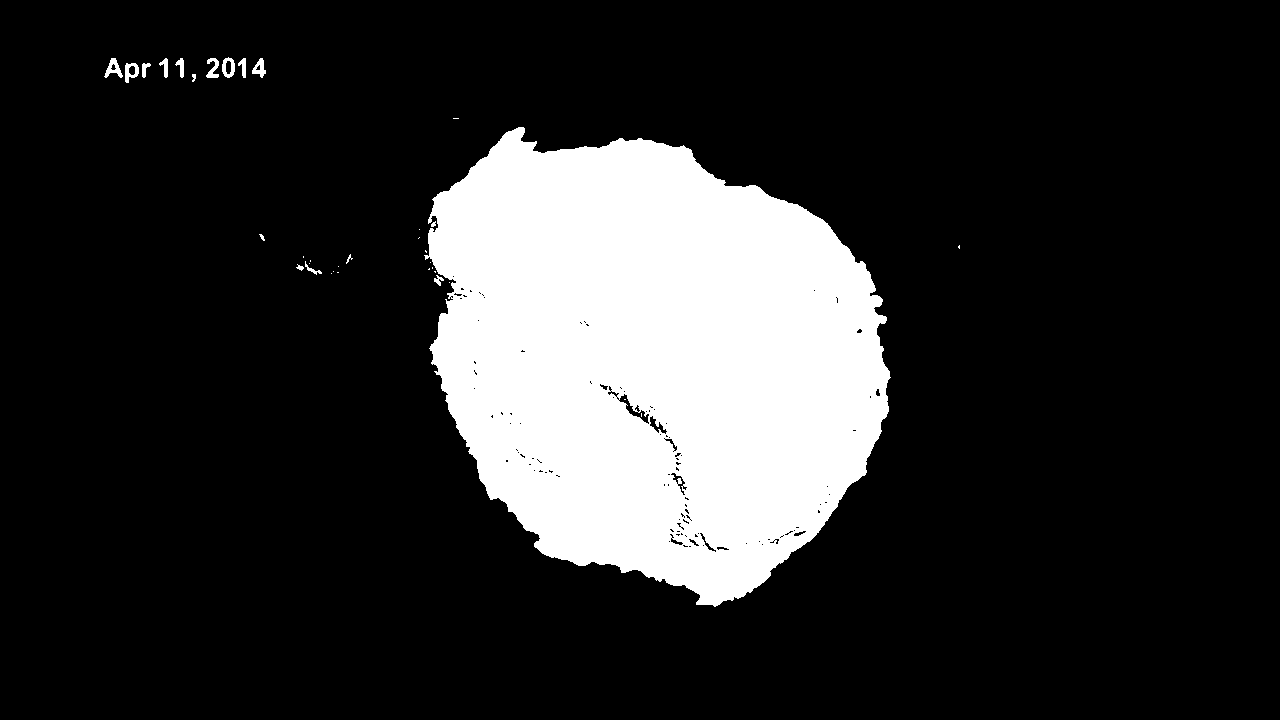
\includegraphics[width=\textwidth]{reportImages/figure2}


\section*{Task 4}
\subsection*{Q6}
I removed the date-stamps from the upper right hand by applying a mask of appropriate size. Having ascertained the pixels required to be removed, I set the values of these pixels in the frame-array manually to zero. 

\subsection*{Fig. 3}
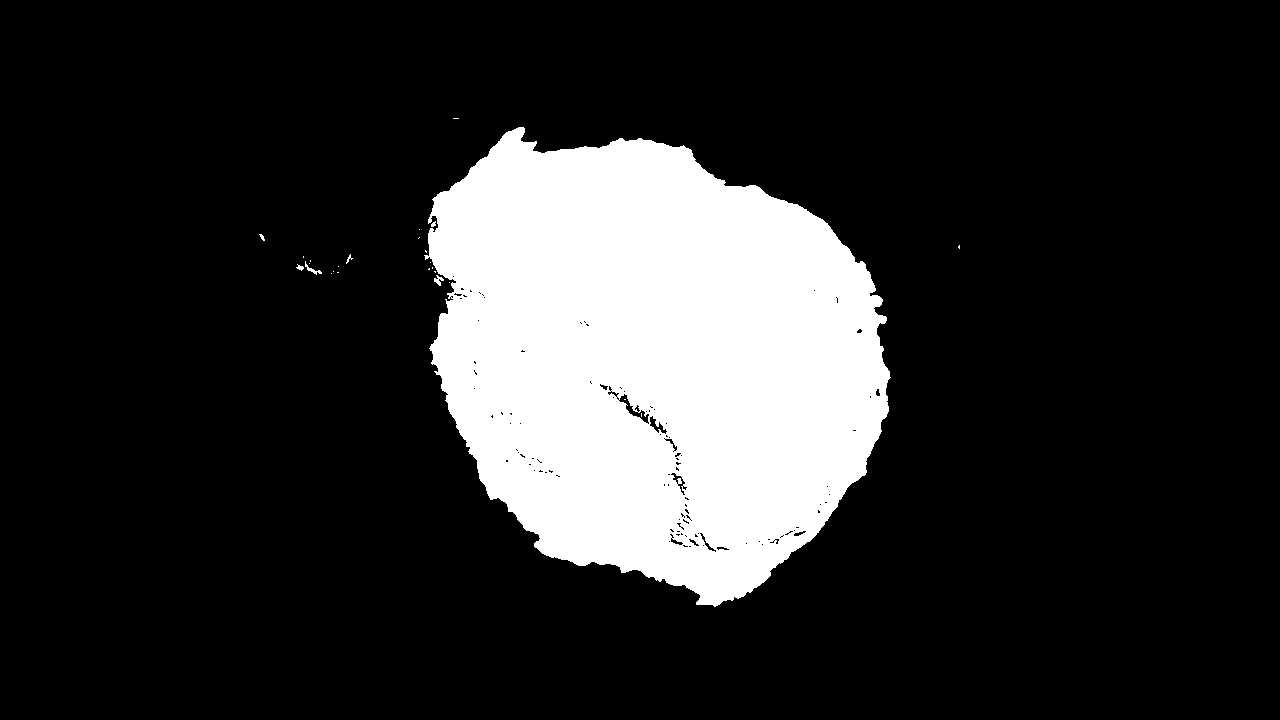
\includegraphics[width=\textwidth]{reportImages/figure3}


\section*{Task 5}
\subsection*{Q7}
\begin{itemize}
	\item I used an averaging-filter of size N=5. 
	\item The filter was applied 5 times for each frame. 
\end{itemize}
\subsection*{Fig. 4}
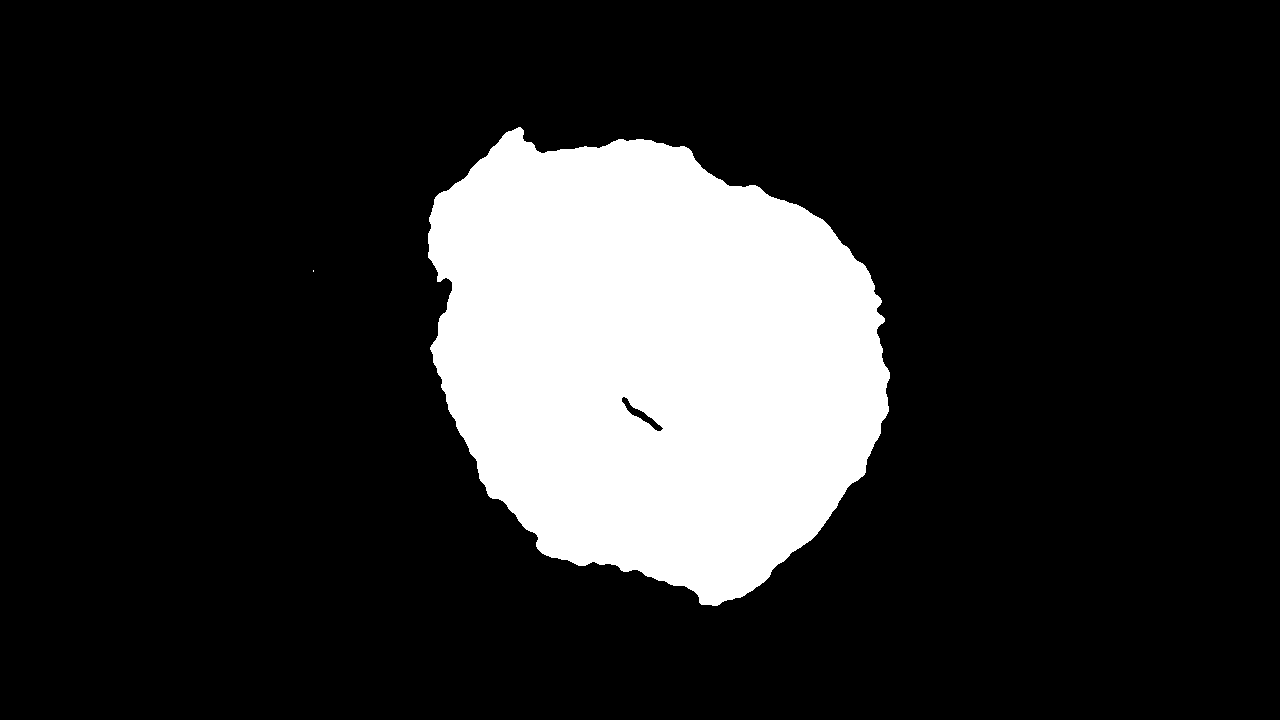
\includegraphics[width=\textwidth]{reportImages/figure4}

\subsection*{Q8}
The discrete Fourier transform of my filter evaluates to one. This is the case for all N. +++

\section*{Task 6}
\subsection*{Fig. 5}

\includegraphics[width=\textwidth]{reportImages/figure5}

\subsection*{Q9}


\section*{Task 7}
\subsection*{Fig. 6}
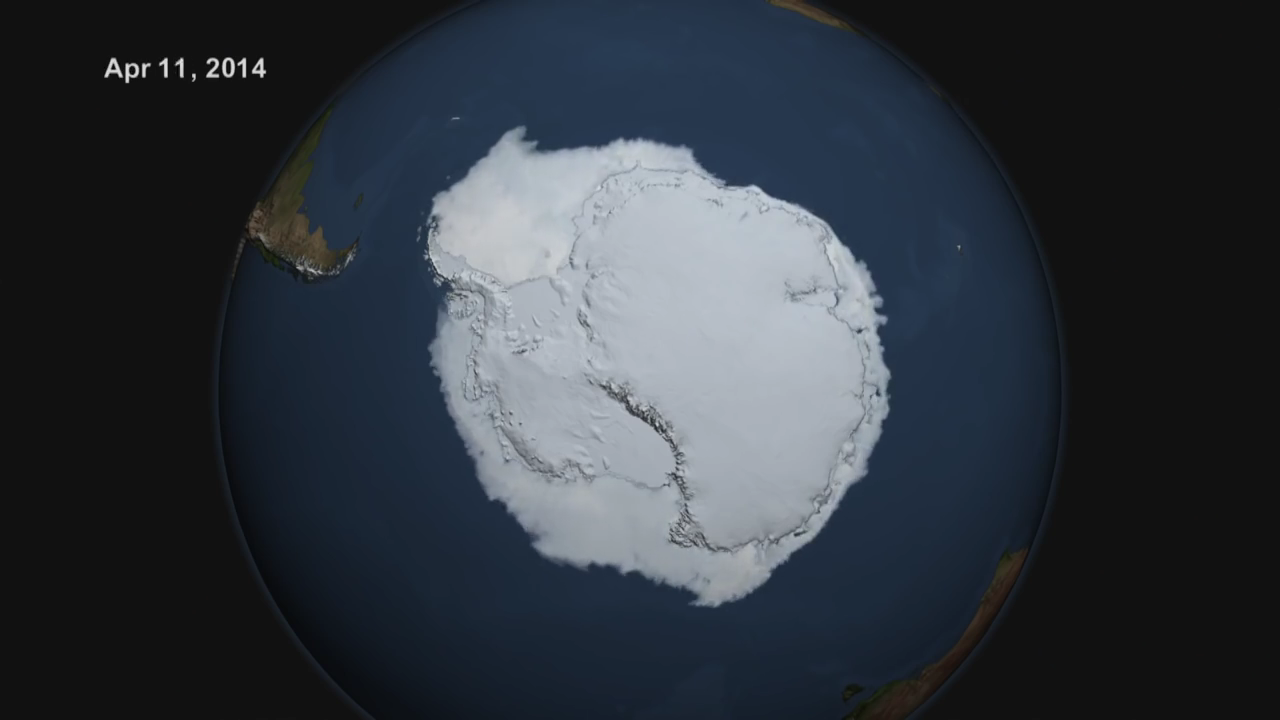
\includegraphics[width=\textwidth]{reportImages/figure6}

\subsection*{Q10}
\subsection*{Q11}

\section*{Task 8}
\subsection*{Fig. 7}
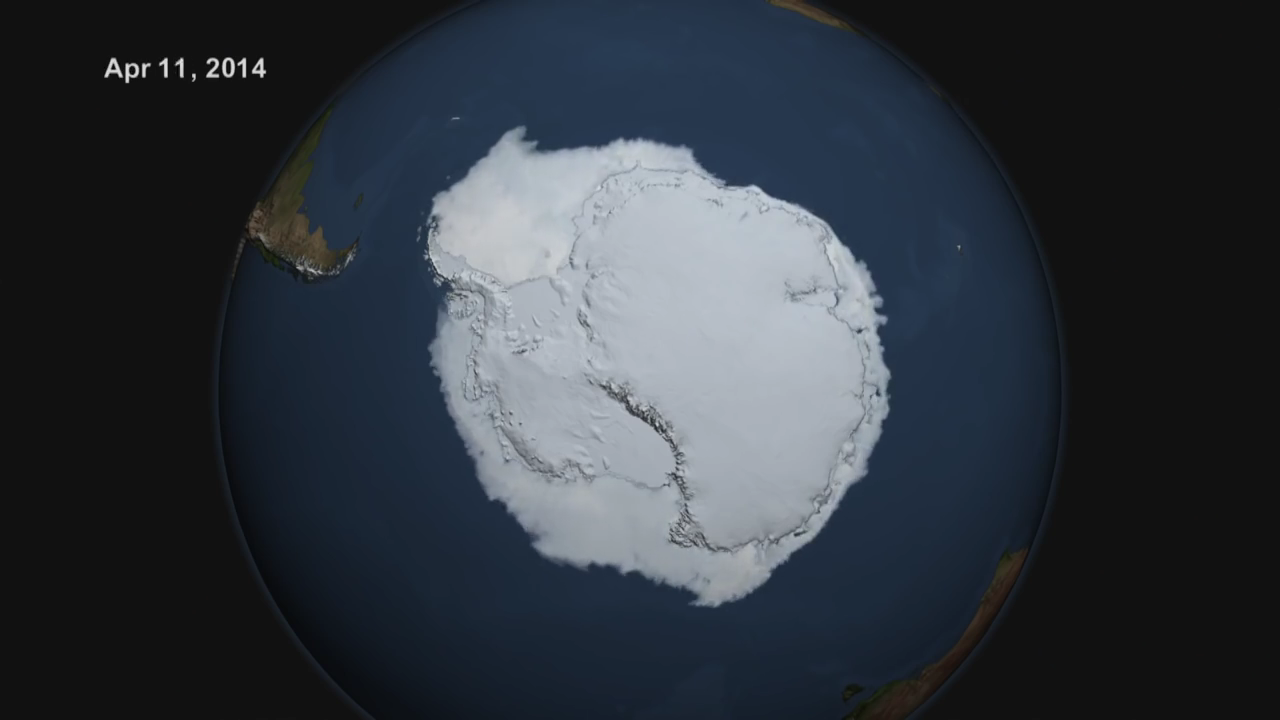
\includegraphics[width=\textwidth]{reportImages/figure7}

\subsection*{Q12}
\subsection*{Fig. 8}
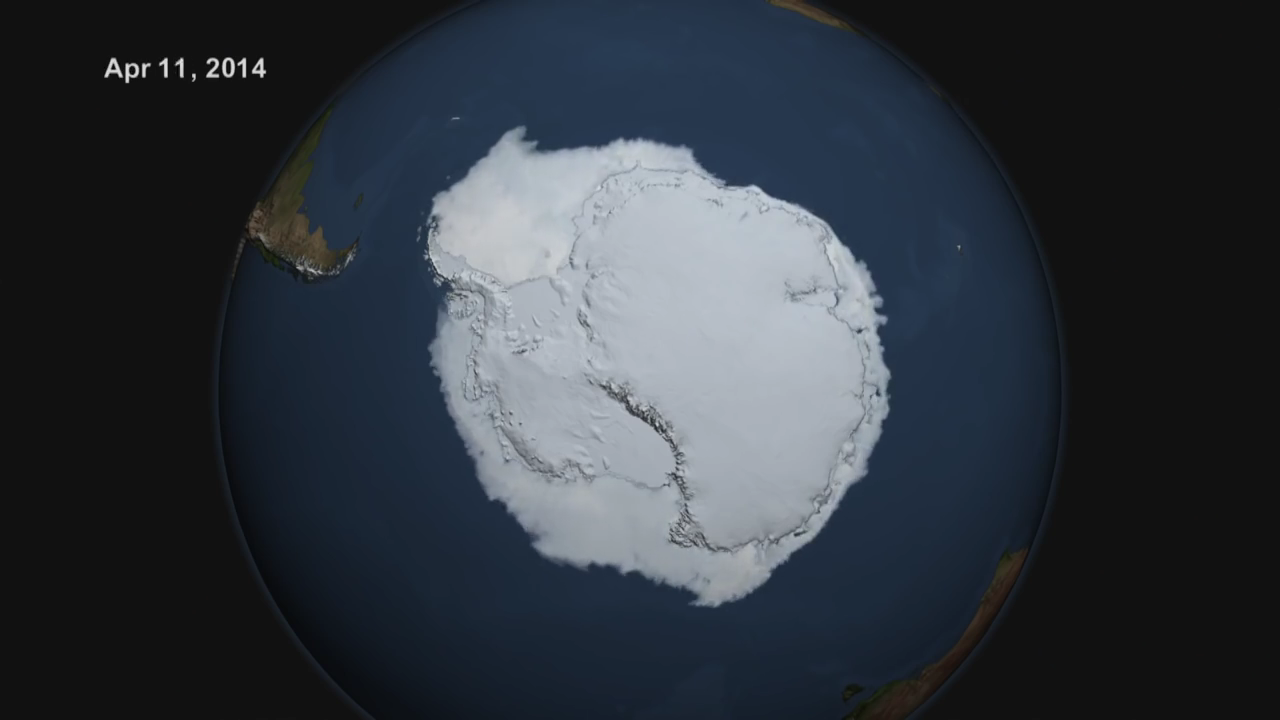
\includegraphics[width=\textwidth]{reportImages/figure8}

\subsection*{Q13}
\subsection*{Q14}

\end{document}
